\section*{Exercício 5}
Ao longo de geodésicas radiais para a luz na métrica de Schwarzschild, temos
\begin{equation*}
    -\left(1 - \frac{2GM}{r}\right)\dl[2]{t} + \left(1 - \frac{2GM}{r}\right)^{-1}\dl[2]{r} = 0,
\end{equation*}
de modo que nestas trajetórias temos
\begin{equation*}
    \left(\diff{t}{r}\right)^2 = \left(1 - \frac{2GM}{r}\right)^2 \implies \diff{t}{r} = \pm \left(1 - \frac{2GM}{r}\right)^{-1}.
\end{equation*}
No limite \(r \to \infty\), temos \(\diff{t}{r} \to \pm 1\), isto é, as trajetórias da luz têm como assíntotas a família de retas \(t = t_0 \pm r\), para constantes \(t_0\). Essa família de retas é a mesma família de geodésicas para o espaço-tempo de Minkowski, isto é, o espaço-tempo dado pela métrica de Schwarzschild é assintoticamente Minkowski.

Resolvendo a equação diferencial, obtemos
\begin{equation*}
    t = \pm r_*(r) + t_0,
\end{equation*}
em que \(t_0\) é uma constante de integração e \(r_*(r)\) é conhecida como a coordenada tartaruga, dada por
\begin{equation*}
    r_*(r) = r + 2GM \ln\abs*{\frac{r}{2GM}-1}.
\end{equation*}
De fato, temos
\begin{equation*}
    \diff{r_*}{r} = 1 + 2GM\frac{\frac1{2GM}}{\frac{r}{2GM}-1} = 1 + \frac{2GM}{r - 2GM} = \frac{r}{r - 2GM} = \left(1 - \frac{2GM}{r}\right)^{-1},
\end{equation*}
portanto a coordenada tartaruga é solução.

% diagrama de espaço-tempo %
% https://www.desmos.com/calculator/aluhj0db7c %
\begin{figure}[ht]
    \centering
    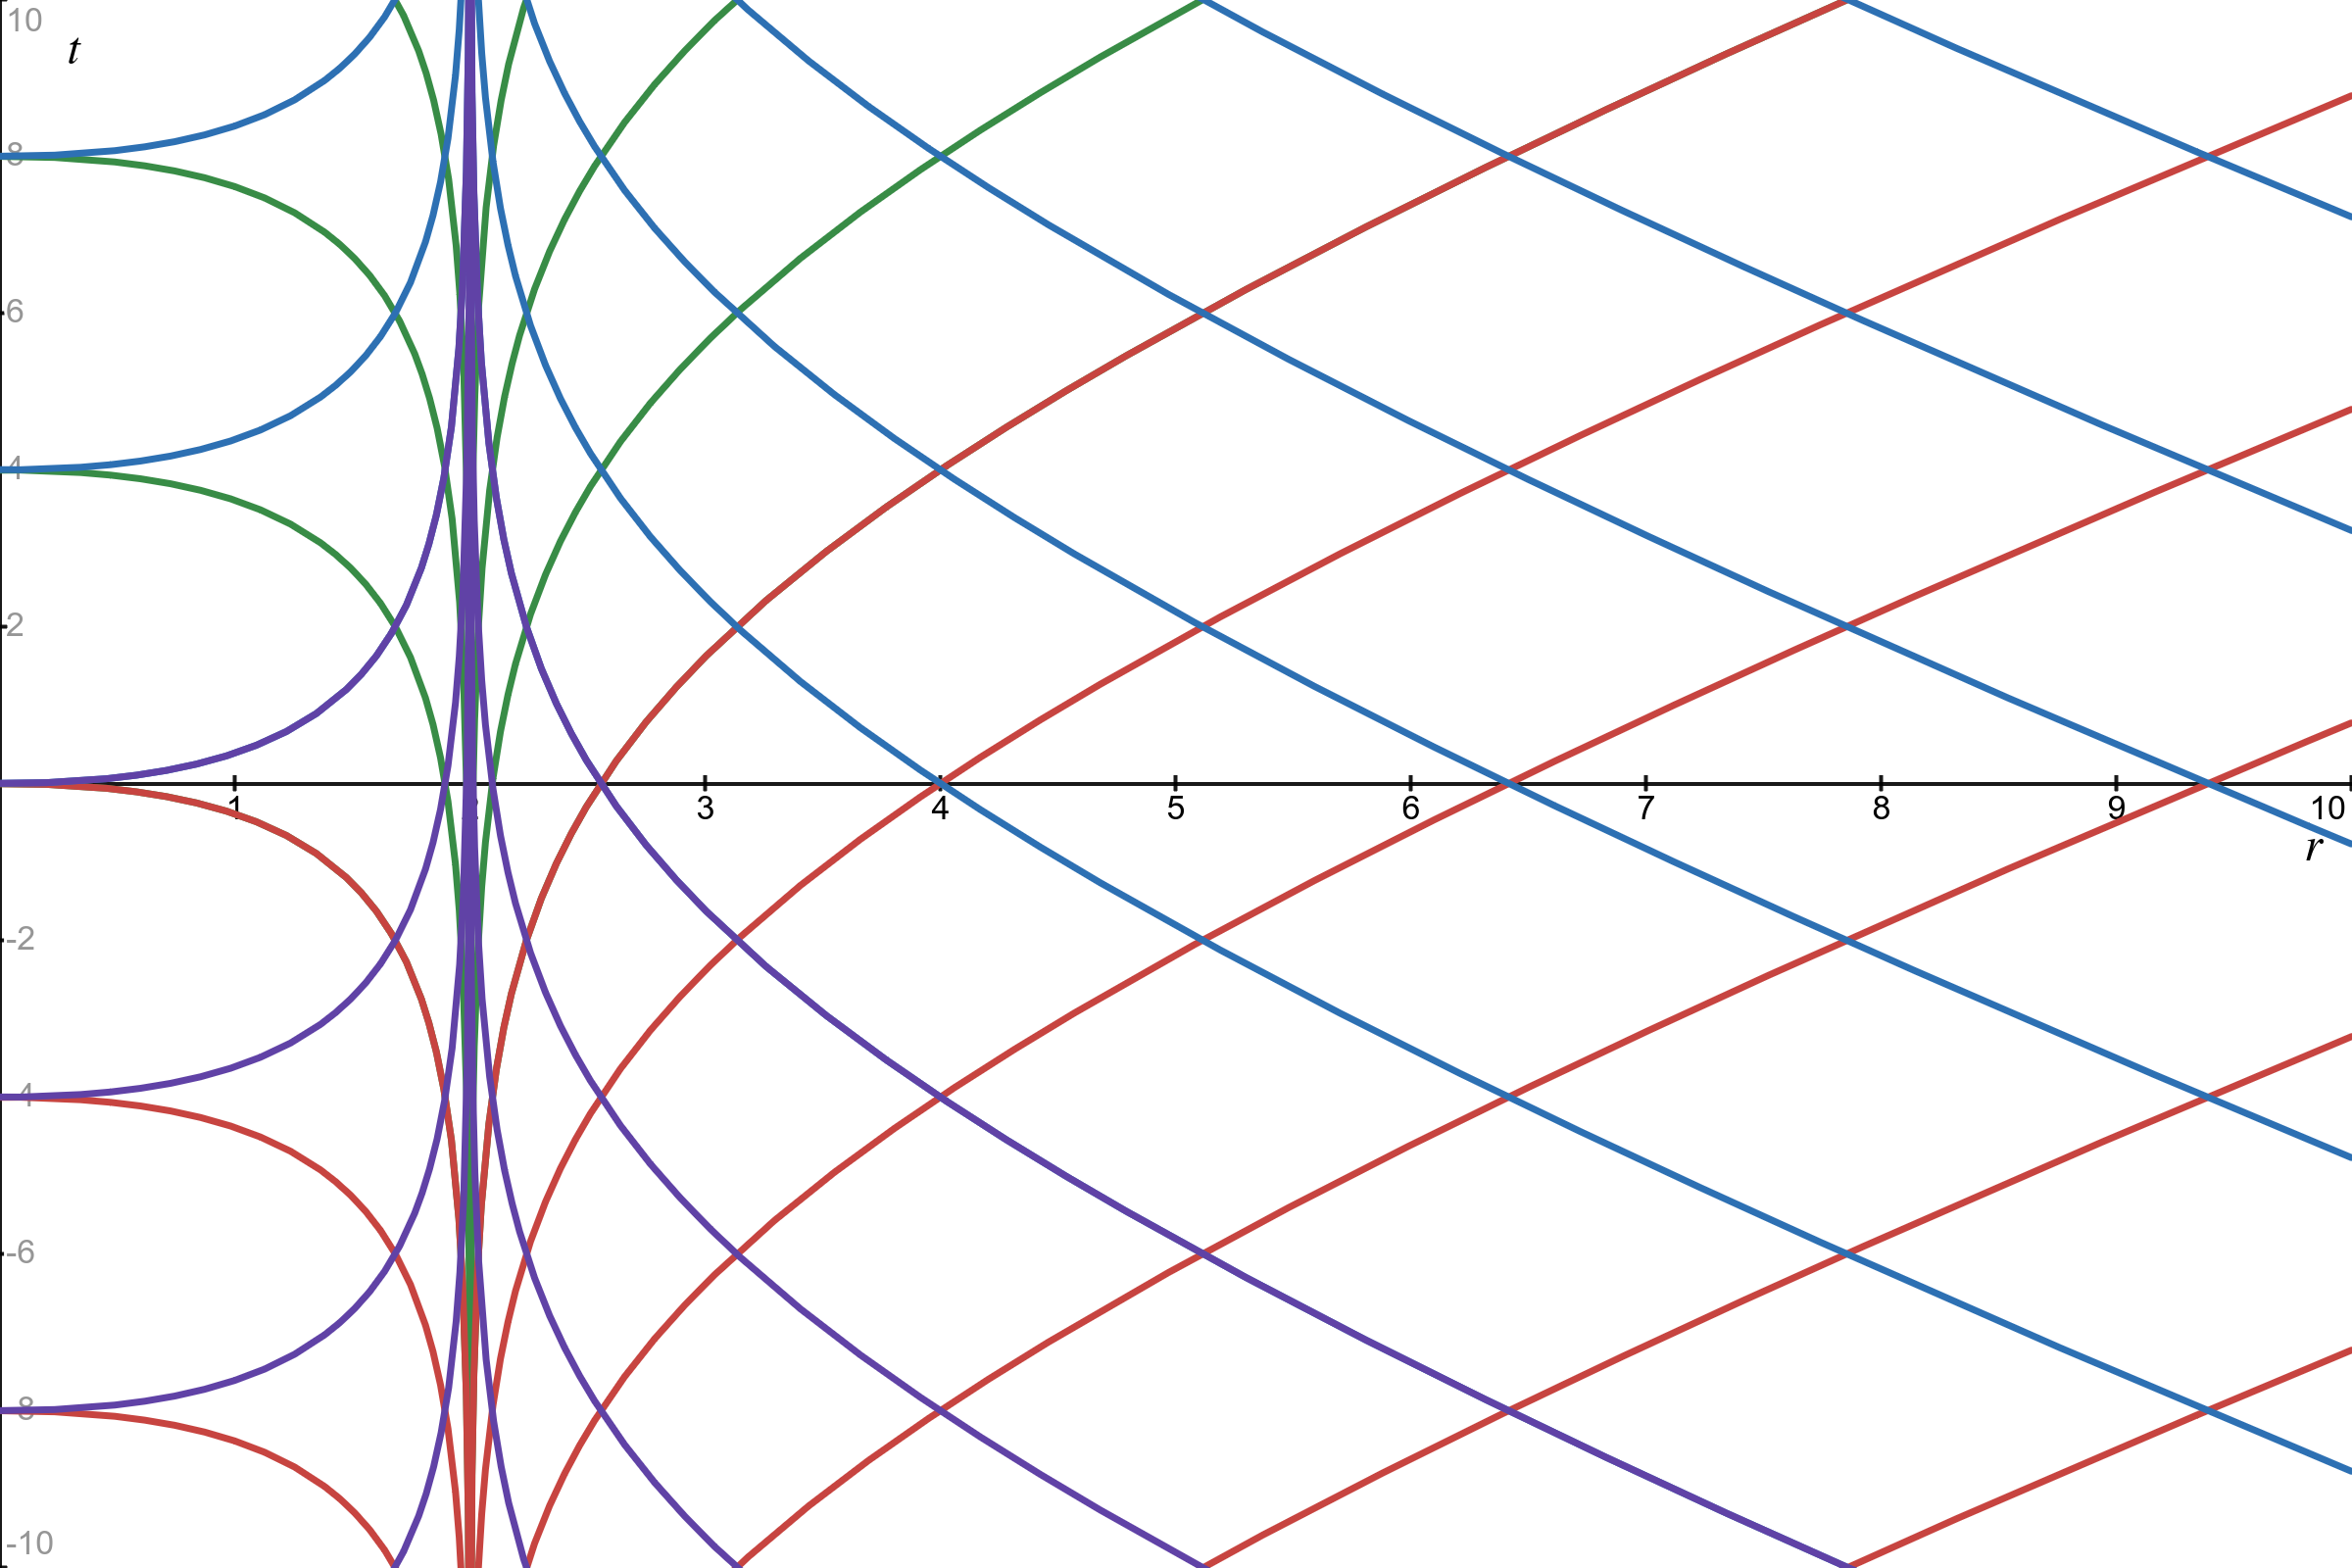
\includegraphics[width=0.6\linewidth]{schwarzschild.png}
    \caption{Diagrama de espaço-tempo nas coordenadas de Schwarzschild com massa unitária.}
    \label{fig:schwarzschild}
\end{figure}

Podemos utilizar a trajetória geodésica encontrada para estender a métrica de Schwarzschild e remover a singularidade das coordenadas em \(r = 2GM\). Primeiro, notemos que
\begin{equation*}
    \lim_{r \to 2GM} r_* = \lim_{r \to 2GM} \left(r + 2GM \ln\abs*{\frac{r}{2GM} - 1}\right) = - \infty,
\end{equation*}
portanto a coordenada tartaruga associa o horizonte de eventos \(r = 2GM\) com \(r_* = -\infty\). Vamos utilizar a trajetória encontrada para a geodésica radial para definir coordenadas
\begin{equation*}
    \left\{\begin{aligned}
        v &= r_*(r) + t\\
        \rho &= r
    \end{aligned}\right. \iff
    \left\{\begin{aligned}
        t &= v - r_*(\rho)\\
        r &= \rho
    \end{aligned}\right.,
\end{equation*}
com as mesmas coordenadas angulares. Nesse caso temos
\begin{align*}
    \diffp{t}{v} &= 1,&\diffp{t}{\rho} &= -\diff{r_*}{r} = - \left(1 - \frac{2GM}{r}\right)^{-1},&\diffp{r}{\rho} &= 1,&\diffp{r}{v} = 0,
\end{align*}
de forma que a métrica nessas coordenadas é dada pelas componentes
\begin{align*}
    \tilde{g}_{vv} &= \left(\diffp{t}{v}\right)^2g_{tt} + \left(\diffp{r}{v}\right)^2g_{rr} = - \left(1 - \frac{2GM}{r}\right)\\
    \tilde{g}_{v\rho} &= \diffp{t}{v}\diffp{t}{\rho} g_{tt} + \diffp{r}{v} \diffp{r}{\rho} g_{rr} = -1\\
    \tilde{g}_{\rho\rho} &= \left(\diffp{t}{\rho}\right)^2 g_{tt} + \left(\diff{r}{\rho}\right)^2 g_{rr} = 0.
\end{align*}
Por motivos psicológicos, renomearemos \(\rho\) para \(r\), de forma que a métrica é dada por
\begin{equation*}
    \dl[2]{s} = -\left(1 - \frac{2GM}{r}\right)\dl[2]{v} + 2\dl{v}\dl{r} + r^2\dl[2]{\Omega},
\end{equation*}
nessas novas coordenadas, chamadas de métrica de Eddington-Finkelstein. Notemos que, nessas coordenadas, temos \(\tilde{g} = \det{\tilde{g_{\mu\nu}}} = r^4\sin^2\theta\), portanto a métrica não é singular em \(r = 2GM\).

% diagrama de espaço-tempo %
% https://www.desmos.com/calculator/giciu2ahe8 %
\begin{figure}[ht]
    \centering
    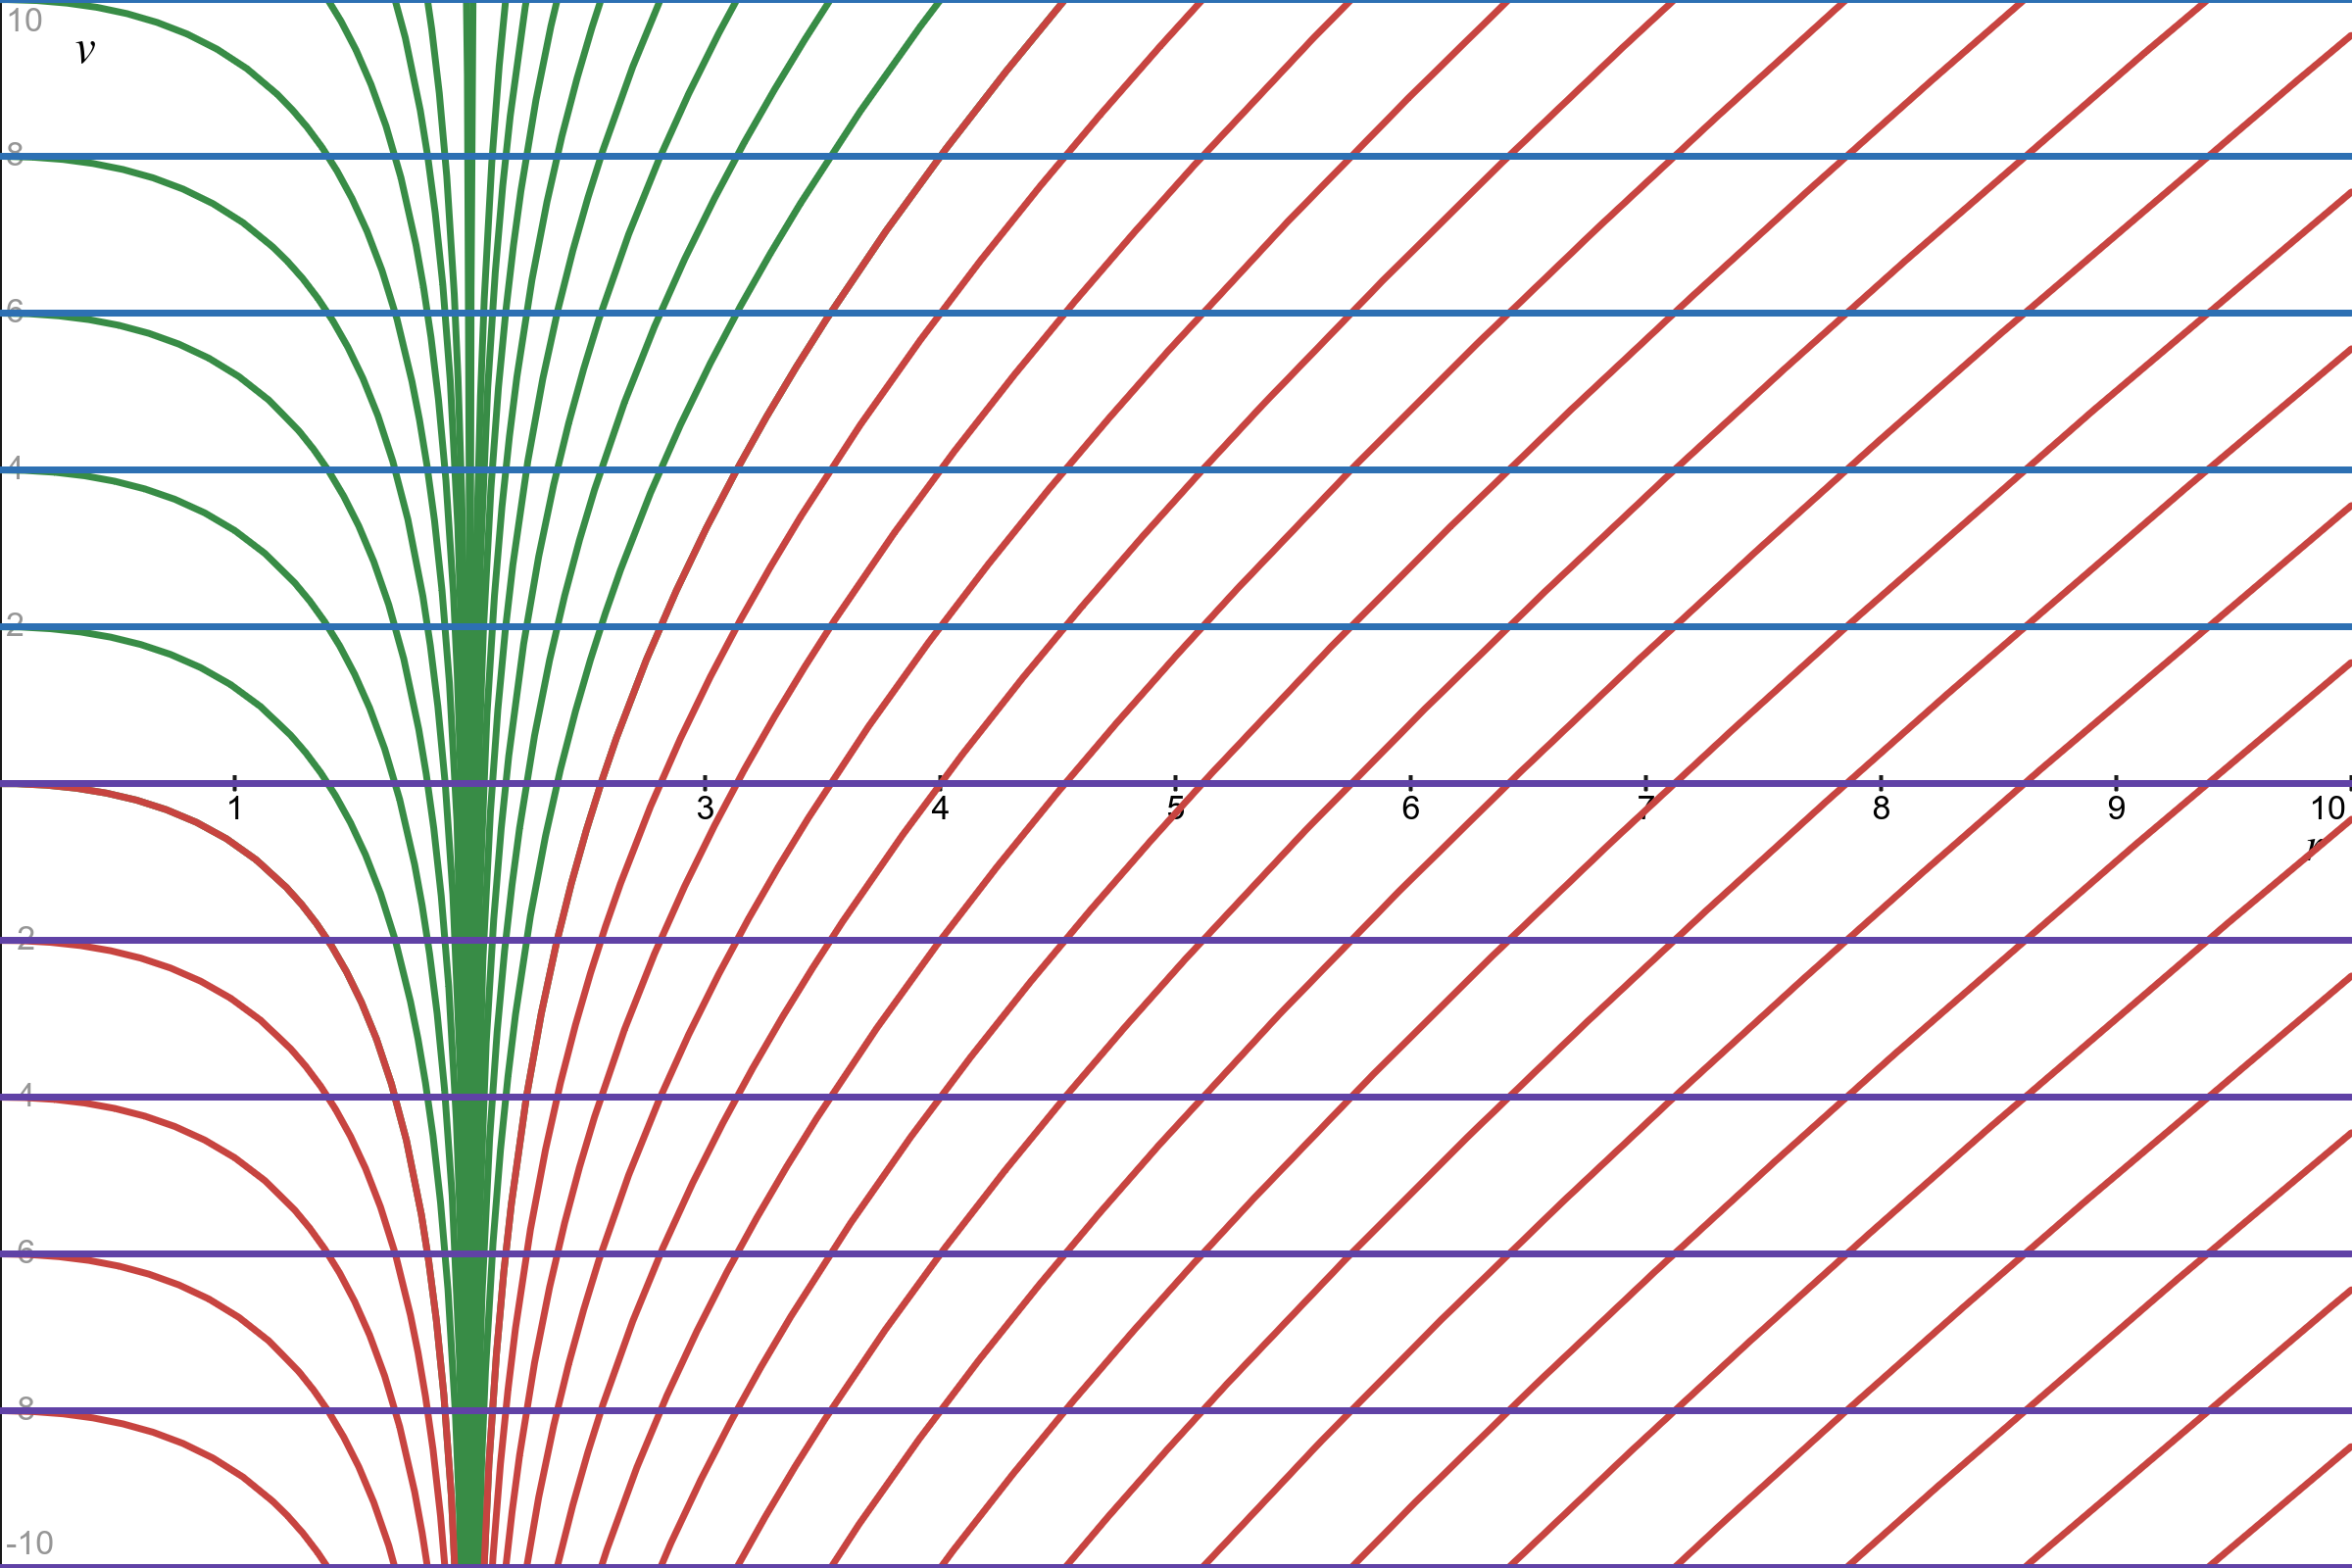
\includegraphics[width=0.6\linewidth]{finkelstein.png}
    \caption{Diagrama de espaço-tempo nas coordenadas de Eddington-Finkelstein com massa unitária.}
    \label{fig:finkelstein}
\end{figure}
